\documentclass{article}
\usepackage[utf8]{inputenc}
\usepackage[T2A]{fontenc}
\usepackage{mathtext}
\usepackage{natbib}
\usepackage{amsmath}
\usepackage{mathtools}
\usepackage{mathptmx}
\usepackage{mathrsfs}
\usepackage{amsfonts}
\usepackage{amssymb}
\usepackage{graphicx}
\usepackage[english, russian]{babel}
\usepackage{hyperref}
\linespread{1.6}
\usepackage[left=1.5cm, right=1.5cm, top=2cm, bottom=2cm, bindingoffset=0cm]{geometry}
\setlength{\parskip}{0.1cm}
\setlength{\parindent}{0.0cm}

\DeclareGraphicsExtensions{.pdf,.png,.jpg}
\usepackage{xcolor}
\definecolor{linkcolor}{HTML}{760B12}
\definecolor{urlcolor}{HTML}{760B12}
\hypersetup{pdfstartview=FitH,  linkcolor=linkcolor,urlcolor=urlcolor, colorlinks=true}


\begin{document}
\large
\tableofcontents % Вывод содержания
\newpage
\section{Введение}
Данный документ является "конспектом".Подразумевается, что читатель ознакомлен с основными
понятиями.

\section{Уравнения}
\subsection{Теория}
Для решения уравнений из второй части ЕГЭ достаточно базовых знаний школьной программы. Наиболее часто используемыми приемами являются: алгебраические
равносильные преобразования, использование 
тригонометрических формул, метод замены переменной. Ниже представлены необходимые тригониметрические формулы:
\\
\[ \sin^2 \alpha + \cos^2 \alpha = 1 \]
\[ 
\sin (\alpha + \beta) = \sin \alpha \cos \beta + \cos \alpha \sin \beta
\]
\[
\sin (\alpha - \beta) = \sin \alpha \cos \beta - \cos \alpha \sin \beta
\]
\[
\cos (\alpha + \beta) =
\cos \alpha \cos \beta - \sin \alpha \sin \beta
\]
\[
\cos (\alpha - \beta) =
\cos \alpha \cos \beta + \sin \alpha \sin \beta
\]
\[
\sin 2\alpha = 2 \sin \alpha \cos \alpha
\]
\[
\cos 2\alpha = 2\cos^2 - 1 = \cos^2 \alpha - \sin^2 \alpha =
1 - 2 \sin^2 \alpha
\]
\\
Выведем всем известную формулу из тригонометрии, а именно \( \cos (\alpha - \beta)\). Отметим на 
тригонометрической окружности две точки $A$ и $B$, каждой из которых соответствует уголи $\alpha$
и $\beta$. 
\begin{figure}[h]
    \center{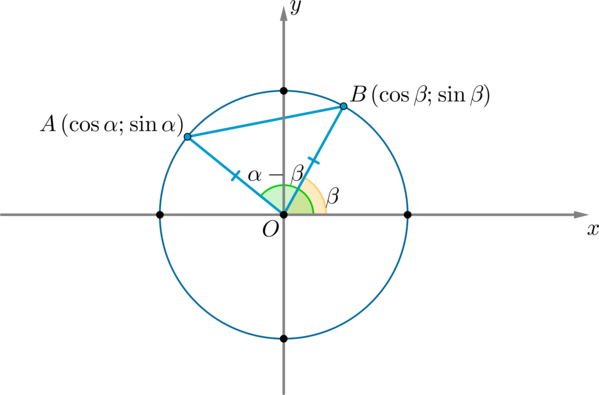
\includegraphics[scale=5.5]{trig_1.png}}
\end{figure}
Координаты точек $A$ и $B$ равны $(\cos \alpha; \sin \alpha)$ и $(\cos \beta; \sin \beta)$ соответственно. 
Для равнобедренного треугольника \( AOB \) применим теорему косинусов относительно угла 
\( \angle AOB = \alpha - \beta \):
\[ AB^2 = AO^2 + OB^2 - 2AO \cdot OB \cos (\alpha - \beta)
\Leftrightarrow AB^2 = 2 - 2\cos (\alpha - \beta)\]
Воспользуемся формулой расстояния между двумя точками:
\[ AB^2 = (\cos \alpha - \cos \beta)^2 + (\sin \alpha - \sin \beta)^2
\Leftrightarrow AB^2 = 2 - 2 \cdot (\cos \alpha \cos \beta + \sin \alpha \sin \beta) \]
Приравниваем полученные уравнения и получаем:
\[ \cos (\alpha - \beta) = \cos \alpha \cos \beta + \sin \alpha \sin \beta \]
Ч. и т.д.
\\
\underline{Упражнение.} Используя формулы приведения, 
выведите косинус суммы, синус разности и синус суммы.
\\
Пару слов про обратные тригонометрическиее функции. 
\[ a = \arcsin x, a \in [-\frac{\pi}{2};\frac{\pi}{2}], x \in [-1;1] 
\Leftrightarrow x = \sin a \]
Арксинус от $x$ -- это такое число в интервале $[-\frac{\pi}{2};\frac{\pi}{2}]$, что синус этого числа равен $x$. 
То есть арксинус -- это функция, обратная к синусу. Очевидно, что если
арксинус принимает в качестве аргумента синус какого-то числа, то множество значений этого аргумента -- это интервал $[-1; 1]$
\\
Аналогично определяется и арккосинус. Ниже представлены графики арксинуса(слева) и арккосинуса(справа)
\begin{figure}[h]
\begin{minipage}[h]{0.49\linewidth}
\center{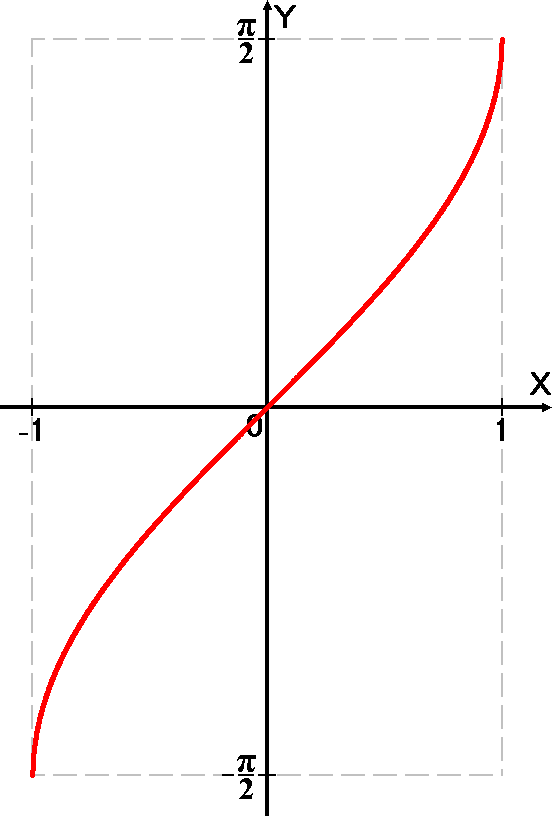
\includegraphics[width=0.5\linewidth]{arcsin.png} \\ y = arcsin x}
\end{minipage}
\begin{minipage}[h]{0.49\linewidth}
\center{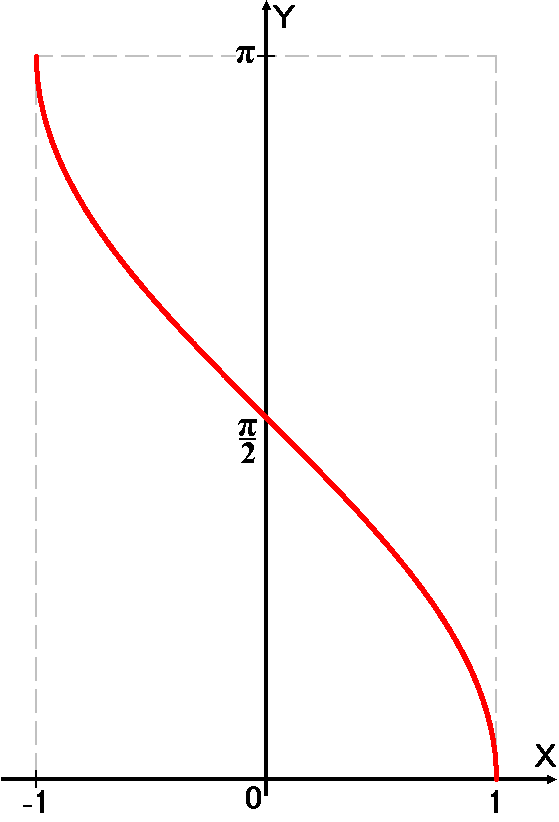
\includegraphics[width=0.5\linewidth]{arccos.png} \\ y = arccos x}
\end{minipage}
\label{ris:image1}
\end{figure}
\[ \arcsin x + \arccos x = \frac{\pi}{2} \]
\[ \arctan x + \arcctg x = \frac{\pi}{2} \]
Доказательство:
\[ \arcsin x = \arcsin (\cos (\arccos x)) = \arcsin (\sin (\frac{\pi}{2} - \arccos x))
= \frac{\pi}{2} - \arccos x\]
\[ \arctan x = \arctan (\ctg (\arcctg x)) = \arctan (\tan(\frac{\pi}{2} - \arcctg x))
 = \frac{\pi}{2} - \arcctg x \]
\\
\underline{Замена переменной}
\\
Иногда(в 13 задаче ЕГЭ это встречается очень часто) мы можем свести
уравнение к более простому виду. Рассмотрим случай:
\[
\sin^2 x + 2 \sin x + 1 = 0
\]
Мы можем решить сначала относительно $\sin x$, потом сделать обратную замену и извлечь итоговый ответ.
\[\sin x = m \]
И уравнение сводится к:
\[m^2 + 2m + 1 = 0
\Leftrightarrow m = -1\]
Делаем обратную замену:
\[
\sin x = -1
\Leftrightarrow
x \in -\frac{\pi}{2} + 2\pi k 
\]
\underline{Линейные уравнения}
\\
Иногда нам может встретиться уравнение следующего 
вида:
\[
p \sin x + q \cos x = r
\]
Если $r = 0$, то все просто:
\[
p \sin x + q \cos x = 0 
\Leftrightarrow
p \sin x = -q \cos x 
\Leftrightarrow
\tg x = - \frac{q}{p}
\]
Если $r \neq 0$, мы можем применить следующее преобразование: разделим обе части на $\sqrt{p^2 + q^2}$
\[
p \sin x + q \cos x = r
\Leftrightarrow
\frac{p}{\sqrt{p^2 + q^2}} \sin x +
\frac{q}{\sqrt{p^2 + q^2}} \cos x = \frac{r}{\sqrt{p^2 + q^2}}
\]
Понятно, что 
\[
\left( \frac{p}{\sqrt{p^2 + q^2}}\right)^2 +
\left( \frac{q}{\sqrt{p^2 + q^2}}\right)^2 =
\frac{p^2 + q^2}{p^2 + q^2} = 1
\]
Таким образом, при синусе и косинусе стоят коэффициенты, которые мы можем представить как 
синус и косинус какого-либо угла. Пусть:
\[
\frac{p}{\sqrt{p^2 + q^2}} = \cos \varphi
\]
\[
\frac{q}{\sqrt{p^2 + q^2}} = \sin \varphi
\]
Таким образом получим:
\[
\cos \varphi \sin x + \sin \varphi \cos x =
\frac{r}{\sqrt{p^2 + q^2}}
\Leftrightarrow
\]
\[
\Leftrightarrow
\sin (x + \varphi) = \frac{r}{\sqrt{p^2 + q^2}}
\]
\\
\underline{Логарифм}
\\
$\log_a b$(произносится как "логарифм $b$ по основанию $a$") -- это такое
число $c$, что $a^c = b$. 
\\
Выражение  \( \log_a b\) определено
тогда и только тогда, когда \underline{\( b > 0\)  и  \( a \in (0; 1) \cup (1;+\infty) \)} 
\\
Логарифмическая является обратной к показательной.
В самом деле, пусть у нас есть \\ \( f(x) = \log_a x \text{ и } g(x) = a^x \). Тогда 
\[ g(f(x)) = a^{\log_a x}  = x \]
\[ f(g(x)) = \log_a a^x = x \log_a a = x \cdot 1 = x \]
При этом \( E_f = \mathbb{R}, D_f = \mathbb{R}_+\) и 
\( E_g = \mathbb{R}_+, D_g = \mathbb{R}\). Что и требовалось доказать 
\\ \\
Пусть\( f(x) = \log_a b \). Тогда если \( a > 1 \), то 
\( f(x) \) возрастает на $\mathbb{R}_+$, если \( a \in (0; 1) \), то
\( f(x) \) убывает на $\mathbb{R}_+$. \\
Действительно, как мы знаем, обратные функции сохраняют монотонность исходной.
\( a^x \) возрастает при $a > 1$ и убывает при \( a \in (0; 1) \). Из этого получаем
монотонность логарифма. \\ 
Основные свойства:
\[ \log_a (x \cdot y) = \log_a x + \log_a y \]
\[ \log_a \frac{x}{y} = \log_a x - \log_a y \]
\[ \log_a x^n = n \cdot \log_a x \]
\[ \log_{y^n} x = \frac{1}{n} \log_y x \] 
\[ \log_y x = \frac{\log_z x}{\log_z y} \]
\[ \log_y x = \frac{1}{\log_x y} \]
\[ z^{\log_y x} = x^{\log_y z} \]
\[ x^{log_x y} = y \]
\subsection{Примеры}
$\mathbf{1}$. Решить уравнение 
\[\cos 2x = \sin\left( x + \frac{\pi}{2}\right)\]
И указать корни, принадлежащие отрезку \( (-2\pi; -\pi)\) \\ \\
\underline{Решение}
\\
Воспользуемся формулами:
\[ 
x = x
\]
$\mathbf{2}$. Решить уравнение
\[ 4 \cos^4 x - 4\cos^2 x + 1 = 0 \]
И указать корни, принадлежащие отрезку \( (-2\pi; -\pi) \) \\ \\
\underline{Решение:} \\
Используем метод замены переменной:
\[ \cos^2 x = m \]
И получим квадратное уравнение тоносительно $m$
\[ 4m^2 - 4m + 1 = 0 
\Leftrightarrow 
(2m - 1)^2 = 0 
\Leftrightarrow
2m - 1 = 0
\Leftrightarrow
m = \frac{1}{2}
\]
Обратная замена:
\[
\cos^2 x = \frac{1}{2}
\Leftrightarrow
\cos x = \pm \sqrt{\frac{1}{2}}
\Leftrightarrow
x = \frac{\pi}{4} + \frac{\pi}{2} \cdot k
\]
\\
$\mathbf{3}$. Решить уравнение
\[ \cos 2x + \sin^2 x = 0,5 \]
И указать корни, принадлежащие отрезку \( [-\frac{7\pi}{2}; -2\pi] \) \\ \\
\underline{Решение}
\\
Воспользуемся формулой косинуса двойного аргумента:
\[
\cos 2x + \sin^2 x = 0,5
\Leftrightarrow
1 - 2\sin^2 x + \sin^2 x = 0,5
\Leftrightarrow
\sin^2 x = \frac{1}{2}
\Leftrightarrow
\sin x = \pm \sqrt{\frac{1}{2}}
\]
$\mathbf{4}$.Решить уравнение
\[ \cos 2x -3\cos x + 2 = 0  \]
И указать корни, принадлежащие отрезку \( [-4\pi; \frac{5\pi}{2}] \) \\ 
\underline{Решение}
\\
\[
\cos 2x -3\cos x + 2 = 0
\Leftrightarrow
2\cos^2 x - 3\cos x + 1 = 0
\]
$\mathbf{5}$. \textit{Решить уравнение}
\[ \frac{3^{\cos x}}{9^{\cos^2 x}} = 4^{2 \cos^2 x - \cos x} \]
И указать корни, принадлежащие отрезку \( [-\frac{3\pi}{2}; \frac{\pi}{6}] \) \\ \\
$\mathbf{6}$. Решить уравнение:
\[ 2\sqrt{3} \sin^2 \left( \frac{3\pi}{2} + x\right) + \sin 2x = 0 \]
\underline{Решение:}
\[ 2\sqrt{3} \sin^2 \left( \frac{3\pi}{2} + x\right) + \sin 2x = 0 
\Leftrightarrow 2\sqrt{3} cos^2 x + 2\sin x \cos x = 0 \]
\[ \Leftrightarrow 2\sqrt{3} \cos x (\cos x + \frac{1}{\sqrt{3}} \sin x) = 0  
\Leftrightarrow \cos x \cdot (\frac{\sqrt{3}}{2} \cos x + \frac{1}{2} \sin x) = 0 \]
\begin{equation*}
    \Leftrightarrow
    \left[
    \begin{gathered}
    \cos x = 0
    \\
    \cos \left( x - \frac{\pi}{6} \right) = 0
    \end{gathered}
    \right.
    \Leftrightarrow 
    \left[
    \begin{gathered}
    x = \frac{\pi}{2} + \pi k
    \\
    x = \frac{2\pi}{3} + \pi k
    \end{gathered}
    \right.
\end{equation*}
\\
$\mathbf{7}$. Решить уравнение:
\[ 6\sin x + 6 \cos 2x = \sin 2x \cdot \cos x + 6\cos^2 x \]
Решение:
\[ 6\sin x + 6 \cos 2x = \sin 2x \cdot \cos x + 6\cos^2 x \]
\[ \Leftrightarrow 6\sin x + 6\cos^2 x - 6\sin^2 x = 2\sin x\cdot \cos^2 x + 6 \cos^2 x  \]
\[ \Leftrightarrow 6\sin x - 6\sin^2 x - 2\sin x \cdot \cos^2 x = 0\]
\[ \Leftrightarrow \sin x \cdot (\sin^2 x - 6\sin x + 4) = 0\]
\begin{equation*}
\Leftrightarrow
    \left[
    \begin{gathered}
    \sin x = 0
    \\
    \sin^2 x - 6\sin x + 4 = 0
    \end{gathered}
    \right.
    \Leftrightarrow
    \left[
    \begin{gathered}
    \sin x = 0
    \\
    \sin x = 1
    \\
    \sin x = 2
    \end{gathered}
    \right.
    \Leftrightarrow
    \left[
    \begin{gathered}
    x = \frac{\pi}{2} + 2\pi k
    \\
    x = \pi k
    \end{gathered}
    \right.
    k \in \mathbb{Z}
\end{equation*}
\\
$\mathbf{8}$. Решить уравнение 
\[ \frac{|\sin x|}{\sin x} + 2 = 2\cdot \cos x\] 
\underline{Решение:}
\begin{equation*}
\frac{|\sin x|}{\sin x} + 2 = 2\cdot \cos x
\Leftrightarrow
    \left[
    \begin{gathered}
    \begin{cases}
    \sin x > 0
    \\
    3 = 2\cos x
    \end{cases}
    \\
    \begin{cases}
    \sin x < 0
    \\
    1 = 2\cos x
    \end{cases}
    \end{gathered}
    \right.
    \Leftrightarrow
    \left[
    \begin{gathered}
    \begin{cases}
    \sin x > 0
    \\
    \cos x = \frac{3}{2}
    \end{cases}
    \\
    \begin{cases}
    \sin x < 0
    \\
    \cos x = \frac{1}{2}
    \end{cases}
    \end{gathered}
    \right.
    \Leftrightarrow
    \begin{cases}
    \sin x < 0
    \\
    x = \pm \frac{\pi}{3} + 2 \pi k, k \in \mathbb{Z}
    \end{cases}
\end{equation*}
\[ \Leftrightarrow x = -\frac{\pi}{3} + 2 \pi k, k \in \mathbb{Z}\]

$\mathbf{9}$. Решить уравнение:
\[ \sin 2x + \cos 2x = 1 \]
\[ \Leftrightarrow 2\sin x \cos x + \cos^2 x - \sin^2 x = \sin^2 x + \cos^2 x 
\Leftrightarrow 2\sin x (\cos x - \sin x) = 0 \Leftrightarrow ...\]

% Блок неравенств 
\section{Неравенства}
\subsection{Теория}
Задача 15, она же неравенства, по своей сложности праетически 
эквивалентна задаче 13. Необходимо уметь работать с логарифмической, показательной, степенной функциями, знать их область определения, область значения, основные свойства. 
\\
\underline{Метод рационализации}
\\
Допустим, нам встретилось подобное неравенство:
\[ \log_{g(x)} f(x) > 0 \]
Мы знаем, что \( \log_{g(x)} f(x) \text{ строго убывает  при } g(x) \in (0;1),  
\text{ строго возрастает при g(x) > 1 }\). Также любой логарифм принимает
нулевой значение только при $f(x) = 1$. Не забывая об ОДЗ, 
запишем все это в виде системы:
\begin{equation*}
    \left[
    \begin{gathered}
    \begin{cases}
    f(x) > 1 \\
    g(x) > 1
    \end{cases}
    \\
    \begin{cases}
    f(x) > 1 \\
    g(x) < 1
    \end{cases}
    \end{gathered}
    \right.
    \Leftrightarrow
    (f(x) - 1) \cdot (g(x) - 1) > 0
\end{equation*}
То есть для решения изначального неравенства достаточно решить систему:
\begin{equation*}
    \begin{cases}
    (f(x) - 1) \cdot (g(x) - 1) > 0 \\
    f(x) > 0 \\
    g(x) > 0 \\
    g(x) \neq 1
    \end{cases}
\end{equation*}
\\
\underline{Упражнение:} Получите аналогичную систему для 
\[
\log_{g(x)} f(x) > 1
\]
\subsection{Примеры}
1. Решить неравенство: 
 \[ 2^{x^2} \leq 4\cdot 2^x\]
 \underline{Решение:}
 \[ 2^{x^2} \leq 4\cdot 2^x \Leftrightarrow 2^{x^2} \leq 2^{x + 2} 
 \Leftrightarrow x^2 \leq x + 2 \Leftrightarrow x^2 - x - 2 \leq 0\]
 \[ \Leftrightarrow (x - 2) \cdot (x + 1) \leq 0 \Leftrightarrow x \in \left[ -1; 2 \right] \]
 
2. Решить неравенство:
\[ 5\cdot 2^{2x + 2} - 21\cdot 2^{x - 1} + 1 \leq 0 \]
\underline{Решение:}
\[ 5\cdot 2^{2x + 2} - 21\cdot 2^{x - 1} + 1 \leq 0 
\Leftrightarrow 20 \cdot 4^x - \frac{21}{2} \cdot 2^x + 1 \leq 0 \]
\[ \Leftrightarrow (2^x - \frac{1}{8})\cdot (2^x - \frac{2}{5}) \leq 0 
\Leftrightarrow 2^x \in \left[ \frac{1}{8}; \frac{2}{5} \right] \]
\[ \Leftrightarrow x \in \left[ -3; \log_2 \frac{2}{5} \right] \]
3. Решить неравенство 
\[ x^{2 - 4\log_2 x + \log^2_2 x} < \frac{1}{x} \]
\underline{Решение:}
\[ x^{2 - 4\log_2 x + \log^2_2 x} < \frac{1}{x} \Leftrightarrow \]
\[ \Leftrightarrow x^{2 - 4\log_2 x + \log^2_2 x} < x^{-1} \]
Как мы знаем, показательная функция $a^x$ возрастает при $a > 1$,
убывает при $0 < a < 1$, и константна при $a = 1$. Так как неравенство строгое,
последний вариант отпадает. Рассмотрим первые два из них: \\
\begin{equation*}
\left[
\begin{gathered}
\begin{cases}
x > 1 \\
2 -4\log_2 x + \log^2_2 x < -1
\end{cases}
\\
\begin{cases}
x \in (0; 1) \\
2 -4\log_2 x + \log^2_2 x > -1
\end{cases}
\end{gathered}
\right.
\Leftrightarrow
\left[
\begin{gathered}
\begin{cases}
x > 1 \\
(\log_2 x - 3) \cdot (\log_2 x - 1) < 0
\end{cases}
\\
\begin{cases}
x \in (0; 1) \\
(\log_2 x - 3) \cdot (\log_2 x - 1) > 0
\end{cases}
\end{gathered}
\right.
\end{equation*}
\\
Дальнейшее решение очевидно.


% Блок параметров

% Блок экономической задачи

\section{Экономическая задача}
\subsection{Примеры}
1. Антон взял кредит в банке на срок 6 месяцев. В конце каждого месяца общая сумма 
оставшегося долга увеличивается на одно и то же число процентов (месячную процентную ставку), а затем уменьшается на сумму, 
уплаченную Антоном. Суммы, выплачиваемые в конце каждого месяца, подбираются так, чтобы в результате сумма долга каждый месяц уменьшалась равномерно, то есть на одну и ту же величину. Общая сумма выплат превысила сумму кредита на 63\%. Найдите месячную процентную ставку.
\\
\underline{Решение.}
\\
Обозначим сумму, взятую в кредит за $S$. По условию нам известно, что сумма долга каждый
месяц уменьшается равномерно, а значит долг ежемесячно уменьшается на \( \frac{S}{6} \). 
Пусть процентная ставка -- $r$\%. Для удобства введем еще одну переменную 
\( \widetilde{r} = 1 + 0,01 \cdot r\). Первая выплата будет составлять 
\( \widetilde{r}S - \frac{5}{6} S\), вторая \( \frac{5}{6} \widetilde{r} S - \frac{4}{6} S\) 
и т.д.
Также по условию нам дана общая сумма выплат, которая составляет
\( 1,63S\).
Вот этих условий нам уже вполне достаточно, чтобы составить уравнение относительно \( \widetilde{r}\):
\[ \left( \widetilde{r}S - \frac{5}{6} S\right)  + 
\left( \frac{5}{6}\widetilde{r}S - \frac{4}{6} S\right) +
\left( \frac{4}{6}\widetilde{r}S - \frac{3}{6} S\right) +
\left( \frac{3}{6}\widetilde{r}S - \frac{2}{6} S\right) +
\left( \frac{2}{6}\widetilde{r}S - \frac{1}{6} S\right) +
\left( \frac{1}{6}\widetilde{r}S - 0\right) = 1,63S \]
\[ \Leftrightarrow \frac{21}{6}\widetilde{r}S - \frac{15}{6}S = 1,63S
\Leftrightarrow \frac{21}{6} \widetilde{r} = 4,13 
\Leftrightarrow \widetilde{r} = 1,18 \Rightarrow r = 18 \]
\underline{Ответ:} \( r = 18\%\)
\\
\\
2. Близнецы Саша и Паша положили в банк по 50 000 рублей на три года под 10\% годовых.
Однако через год и Саша, и Паша сняли со своих счетов соответственно 10\% и 20\% имеющихся денег. 
Еще через год каждый из них снял со своего счета соответственно 20 000 рублей и 15 000 рублей. 
У кого из братьев к концу третьего года на счету окажется большая сумма денег? На сколько рублей?
\\
\\
3. Владимир поместил в банк 3600 тысяч рублей под 10\% 
годовых. В конце каждого из первых двух лет хранения после 
начисления процентов он дополнительно вносил на счет одну и 
ту же фиксированную сумму. К концу третьего года после 
начисления процентов оказалось, что размер вклада увеличился 
по сравнению с первоначальным на 48,5\%. Какую сумму Владимир
ежегодно добавлял к вкладу?
\\
\underline{Решение:}
\\
Ну тут ситуация совсем простая. Обозначим добавленную сумму за \( \Delta S\). В конце первого
года послу начисления процентов и добавления неизвестной суммы вклад будет равен 
\( 1,1\cdot 3600 + \Delta S = 3960 + \Delta S\), в конце второго: 
\( 1,1\cdot (3960 + \Delta S) + \Delta S \), в конце третьего года:
\[ 1,1 \cdot ( 1,1\cdot (3960 + \Delta S) + \Delta S) = 1,486 \cdot 3600 \]
\[ \Leftrightarrow 4791,6 + 2,31 \cdot \Delta S = 5346 
\Leftrightarrow \Delta S = 240 \]
\underline{Ответ:} 240 тысяч рублей
\\
\\
4. В июле планируется взять кредит в банке на сумму 18 млн рублей на некоторый срок (целое число лет). Условия его возврата таковы:\\
— каждый январь долг возрастает на 10\% по сравнению с концом предыдущего года;
\\
— с февраля по июнь каждого года необходимо выплатить часть долга;
\\
— в июле каждого года долг должен быть на одну и ту же сумму меньше долга на июль предыдущего года.
\\
На сколько лет был взят кредит, если общая сумма выплат после полного погашения кредита составила 27 млн рублей?
\\
\underline{Решение:}
\\
Пусть количество лет -- это $n$. Как будет меняться сумма долга в июле каждого года:
\[ S, \frac{n-1}{n} \cdot S; \frac{n-2}{n} \cdot S; ... \frac{S}{n}; 0 \]
Каждый январь долг возрастает на 10\%, и будет составлять:
\[ 1,1 \cdot S; 1,1 \cdot\frac{n-1}{n}S; 1,1\cdot \frac{n-2}{n}  S; ... 1,1 \cdot \frac{S}{n}; 0\]
Выплаты складываются из процентов и величины \( \frac{S}{n}\), на которую долг убывает каждый июль.
Значит итоговые выплаты:
\[ n\cdot \frac{S}{n} + 0,1 \cdot 18\cdot \left( \frac{1}{n} + ... + \frac{n - 1}{n} +
\frac{n}{n}\right) =  18 + 18 \cdot 0,1 \cdot \frac{n + 1}{2} = 27
\Leftrightarrow n = 9\]
\underline{Ответ:} n = 9
\\
\\
5. В июле 2020 года планируется взять кредит на некоторую сумму. Условия возврата таковы:
\\
— в январе каждого года долг увеличивается на 30\% по сравнению с предыдущим годом;
\\
— с февраля по июнь нужно выплатить часть долга одним платежом.
\\
Определите, на какую сумму взяли кредит банке, если известно, что кредит был выплачен тремя равными платежами (за 3 года) и общая сумма выплат на 156 060 рублей больше суммы взятого кредита.
\\
\underline{Решение}
\\
Положим, что кааждая из трех выпла равняется $x$, Сумма долга(изначальная) -- $S$. 
\\
Согласно условию, общая сумма выплат на 156 060 рублей больше суммы взятого кредита:
\[ 3x = S + 156060 \]
Теперь запишем уравнение для выплат. Сначала сумма долга возрастает в 1.3 раза, далее выплачивается доля $x$, и так
три раза, при этом в конце сумма долга равна нулю.
\[
    1,3(1,3(S - x) - x) - x = 0
\]
\\
\underline{Ответ:} 239400 рублей
\\ \\
6. Светлана Михайловна взяла кредит в банке на 4 года на сумму 4 420 000 рублей. 
Условия возврата кредита таковы: в конце каждого года банк увеличивает текущую сумму долга на 10 \%. 
Светлана Михайловна хочет выплатить весь долг двумя равными платежами ― в конце второго и четвертого годов. 
При этом платежи в каждом случае выплачиваются после начисления процентов. Сколько рублей составит каждый из этих платежей?
\underline{Ответ:} 2928200 рублей
\\ \\
7. 15-го декабря планируется взят кредит в банке на 1 000 000 рублей на (n + 1) месяц. Условия его возврата таковы:
\\
— 1-го числа каждого месяца долг возрастает на r\% по сравнению с концом предыдущего месяца;
\\
— cо 2-го по 14-е число каждого месяца необходимо выплатить часть долга;
\\
— 15-го числа каждого месяца с 1-го по n-й долг должен быть на 40 тысяч рублей меньше долга на 15-е число предыдущего месяца;
\\
— 15-го числа n-го месяца долг составит 200 тысяч рублей;
\\
— к 15-му числу (n + 1)-го месяца кредит должен быть полностью погашен.
\\
Найдите r, если известно, что общая сумма выплат после полного погашения кредита составит 1378 тысяч рублей.

\underline{Краткое решение:}
Из условия задаром получим $n$. Первые $n$ месяцев долг убывает следующим образом:
\[ 1000, 960, 920...240, 200\]
\[ n = \frac{1000 - 200}{40} = 20\]
Введем для удобства \( \widetilde{r} = 1 + \frac{r}{100} \)
Размер долга на первое число будует составлять:
\[ 1000\cdot \widetilde{r}...200\cdot \widetilde{r}\]
Можем посчитать выплаты:
\[ (\widetilde{r} - 1)1000 + 40...(\widetilde{r} - 1)240 + 40, 200 \widetilde{r} \]
Общая сумма выплат составит:
\[ 12600 \widetilde{r} - 11600 = 1378 \Rightarrow \widetilde{r} = 1,03\]
\underline{Ответ:} \( r = 3\)
\\ \\

\section{Задачи с параметром}
\subsection{Теория}
Несмотря на то, что задача с парамером не требует каких либо внешкольных знаний, данный раздел являеся наиболее объемным, и, пожалуй, наиболее сложным для осознания и воспрятия читателем. В средней общеобразовательной школе
подобного рода задачам либо не уделяют внимания вообще, либо разбирают их крайне поверхностно. В общем виде уравнение, содержащее параметр, выглядит так:
\[ F(x, a) = 0 \]
Конечно, это может быть и неравенство, и система неравенств, и система уравнений, но мы начнем обсуждение с самого простого случая. В приведенном выше уравнении содержатся переменная $x$ и параметр $a$, который может принимать различные значения. 
\\
Если перед нами стоит задача решить уравнение с параметром,
то мы представляем, что $a$ -- это обычное вещественное 
число, но какое конкретно -- нам неизвестно. Очевидно, что 
он может влиять как на то, какими будут корни уравнения. Обычно мы не рассматривает параметр как 
переменную, хотя в некоторых случаях это позволяет упросить 
решение(В дальнейшем этот вопрос будет раскрыт более 
подробно).
Разберем простейший, но достаточно наглядный пример:
\[
x^2 - a = 0
\]
Что равносильно:
\[
x^2 = a
\]
Понятно, что если $a < 0$, то вещественных корней у этого
уравнения нет(квадрат не может принимать отрицательные
значения). В случае $a = 0$ получаем, что $x = 0$. А если
$a > 0$, то образуются два корня: $x = \pm \sqrt{a}$.
\\
Разберем еще один пример. Решим уравнение в двумя параметрами:
\[
ax + b = 0
\]
Очевидно, что если ни $a \neq 0$, то $x = 
-\frac{b}{a}$. Если $a = 0$ и $b = 0$, то получим:
\[0 \cdot x + 0 = 0 \]
Что верно при всех $x \in R$. В случае $a=0,b\neq 0$ получим, что $x \in \varnothing$. 
\\
\\
В некоторых случаях для решения задачи необходимо построить
график сложной функции.
\\
\begin{center}
\begin{tabular}{| l | l |}
\hline
     \( y = f(x) + a\) &  параллельный перенос вдоль оси Oy \\ \hline
     \( y = f(x + a) \) & параллельный перенос вдоль оси Ox \\ 
      & \( a > 0 \quad \leftarrow \) \\
      & \( a < 0 \quad \rightarrow \) \\ \hline 
      \( y = |f(x)| \) & Симметрия нижней части графика относительно оси Ox \\
      & \( f(x), f(x) \geq 0\) \\
      & \( -f(x), f(x) \leq 0\) \\ \hline
      \(y = -f(x)\) & Симметрия графика относительно Ox \\ \hline
      \( y = f(-x) \) & Симметрия графика относительно Oy \\ \hline
      \( y = f(|x|) \) & Все, что правее оси Oy, не изменяется \\
      & Все, что левее оси Oy, стирается, \\
      & а вместо нее появдяется график, \\
      & симметричный правой части относительно Oy \\ \hline
      \( y = af(x), a > 0 \) & Растяжение относительно Ox в $a$ раз \\ \hline
      \( y = f(ax) \) & Сужение относительно Oy в $a$ раз \\ \hline
\end{tabular}
\end{center}
\underline{Теория функций}
\\
\underline{Определение} Пусть заданы два множества $X$ и $Y$. Говорят, что задана функция(отображение) $f: X \rightarrow Y$, если каждому элементу из $X$ ставится
в соответствие единственный элемент из $Y$. При этом множество $X$ --
это область определения, и обозначается как $D(f)$, а множество:
\[ E(f) = \left\{ f(x)| x \in X \right\} \]
Называется множество значений функции $f$.
\\
Пример: 
\\
$f(x) = x^2$. Область определения -- $\mathbb{R}$, множество значений -- $[0; +\infty)$
\\
$f(x) = x^3$. Область определения -- $\mathbb{R}$, множество значений -- $\mathbb{R}$
\\ $f(x) = \log_2 x$. Область определения -- $(0; +\infty)$, множество 
значений -- $\mathbb{R}$.
\\
\\
Функция называется непрерывной, если:
\[\lim_{x \rightarrow x_0} f(x) = f(x_0) \quad \forall x \in D(f)\]
Интуитивно мы можем представить это так: функция непрерывна на промежутке, если ее график на этом промежутке можно нарисовать, не отрывая руки.
\\
Напоминаю, что предел функции по определению:
\[
\lim_{x \rightarrow x_0} f(x) = a
\Leftrightarrow
\forall \epsilon > 0 \exists \delta: \forall x, |x - x_0| < \delta: |f(x) - a| < \epsilon
\]
Производная функции:
\[
f'(x_0) = \lim_{x \rightarrow x_0}
\frac{f(x) - f(x_0)}{x - x_0}
\]
\[
f' = \frac{df}{dx}
\]
То есть это отношение приращения функции к приращению аргумента. При этом:
\[
df = f' \cdot dx
\]
Называется дифференциалом $f$.
\\
Смысл производной состоит в том, что она показывает скорость возрастания $f$. Также она являеся тангенсом угла касательной, проведенной в точке $x_0$, и это можно понять интуитивно, ведь приращение функции и приращение аргумента -- это противолежащий и прилежащий катеты соответственно, а касательная приблизается к функции при бесконечном приближении к точке $x_0$
\subsection{Примеры}
\underline{1} При каких $a$ система имеет ровно 4 решения.
\[
\begin{cases}
(x - 2a - 2)^2 + (y - a)^2 = 1
\\
y^2 = x^2
\end{cases}
\]
Второе уравнение в системе равносильно: $|x| = |y|$, значит возможны два случая:
\[ 
\left[
\begin{gathered}
x = y
\\
x = -y
\end{gathered}
\right.
\]
Заметим следующее: для каждого из этих вариантов по отдельности первое
уравнение имеет максимум два решения(так как при подстановке $x = y$ или $x =- -y$ оно, очевидно, станет квадратным). Значит, чтобы система имела ровно четыре решения, нужно, чтобы в первом случае($x = y$) первое уравнение имело два корня, во втором случае($y = -x$) первое уравнение имело два корня, и при этом корни не совпадали. 
\\
1) Подставим $x = y$ в первое уравнение:
\[ x^2 - 2(2a + 2) x + 4a^2 + 8a + 4 + x^2 - 2ax + a^2 = 1 \Leftrightarrow 
2x^2 - 2(3a + 2)x + (2a + 2)^2 + a^2 - 1 = 0 \]
Уравнение имеет два корня, следовательно:
\[ D = -4(a^2 + 4a + 2) > 0 \Leftrightarrow a^2 + 4a + 2 < 0 \Leftrightarrow 
a \in (-2 - \sqrt{2}; -2 + \sqrt{2}) \]
2) Подставим $x = -y$ во второе уравнение:
\[ 2x^2 - 2(a + 2)x (2a + 2)^2 + a^2 - 1 = 0 \]
Уравнение имеет два корня, следовательно:
\[ D = -4(9a^2 + 12a + 2) > 0 \Leftrightarrow  9a^2 + 12a + 2 > 0 
\Leftrightarrow a \in (\frac{-2 -\sqrt{2}}{3}; \frac{-2 + \sqrt{2}}{3}) \]
Также нужно проверить, что решения не совпадают. Пусть есть некий общий корень $x_0$. Подставим в уравнения и приравняем:
\[ 2x_0^2 - 2(3a + 2)x_0 + (2a + 2)^2 + a^2 - 1 = 2x_0^2 - 2(2 + a)x_0 + (2a + 2)^2 + a^2 - 1  
\Leftrightarrow (2a + 2)^2 + a^2 - 1 = 0 \]
\[ \Leftrightarrow 
\left[
\begin{gathered}
a = -1 
\\
a = -0,6
\end{gathered}
\right.
\]
То есть при данных значениях параметра $a$ корни уравнений будут совпадать, что нам не подходит.
\\
Далее объединим первые два интервала и учтем условие $a \neq -1, a \neq -0,6$
\\
По итогу:
\[
\begin{cases}
a \in (-2 -\sqrt{2}; -2 + \sqrt{2})
\\
a \in (\frac{-2 - \sqrt{2}}{3};\frac{2 + \sqrt{2}}{3})
\\
a \neq -0,6
\\
a \neq -1
\end{cases}
\Leftrightarrow
\underline{a \in (\frac{-2 - \sqrt{2}}{3}; -1) \cup (-1, -0,6) \cup (-0,6; -2 + \sqrt{2})}
\]
\end{document}